\chapter{Design and implementation}
In this chapter we delve into the design and the implementation details of
\TOOL, the tool we built to generate SEFL models from iptables configurations
with the end goal of having them embedded in complex networks which can then be
verified using SymNet.

We begin with a high-level outline of the computation steps that take place
between dumping iptables configurations to returning a model as expected by
SymNet.  Following that, we take each of those steps separately and discuss the
most important aspects of their implementation details.  At the end we go into
more details about a few extensions to illustrate how straightforward it is to
add new ones, both structurally and logically.


\section{Design overview}

\TOOL is essentially a compiler: its input is a file that aggregates per-table
rules dumped by the \emph{iptables} command line tool, and it outputs two Map
data structures expected by SymNet, one for port connections and the other for
port instructions (\labelindexref{Section}{sec:first-steps}).  Alternatively,
it can return a Scala object modelling the whole device if integration with
other network components is desired.

Driven by this observation, we designed \TOOL to mimic the internal
structure of a compiler too; it features three separate, well-defined phases:
\begin{itemize}
  \item \textbf{Parsing}. The input file is read and an in-memory Abstract
    Syntax Tree (AST)\abbrev{AST}{Abstract Syntax Tree} is built.  It
    materializes the hierarchy shown in
    \labelindexref{Figure}{fig:iptables-hierarchy}.
  \item \textbf{Validation}.  This step resembles \emph{semantic analysis} in
    usual compilers and its purpose is twofold:
    \begin{enumerate*}[i)]
      \item ensures that the configurations conform to the official
        specifications, and
      \item augments the AST with additional semantic information that either
        could not be gathered during parsing or it yields a more robust design
        to do it now.
    \end{enumerate*}
  \item \textbf{Code generation}. This phase is essential in any compiler and
    ours is no exception: based on the now validated in-memory AST we generate
    SEFL code for every rule as a two step process: first generate the
    constraints that correspond to rule's matches, and then
    generate the code to follow its target.

    In addition to that, we also consider as part of this step putting all
    things together according to the model template devised in the previous
    chapter (\labelindexref{Figure}{fig:iptables-2} and
    \labelindexref{Figure}{fig:chain-internal}).  We call it a \emph{template}
    because it is only a model once we fill it with real rules.  In fact, this
    step is similar to the \emph{backend} component in a compiler that is tied
    to a concrete machine architecture instead of an abstract one.  Until this
    step, the AST is a simplified and better organized view of the input rules
    but it still abstract enough to target various table/chain structures.
\end{itemize}

\begin{figure}[h]
  \centering
  \captionsetup{justification=centering}
  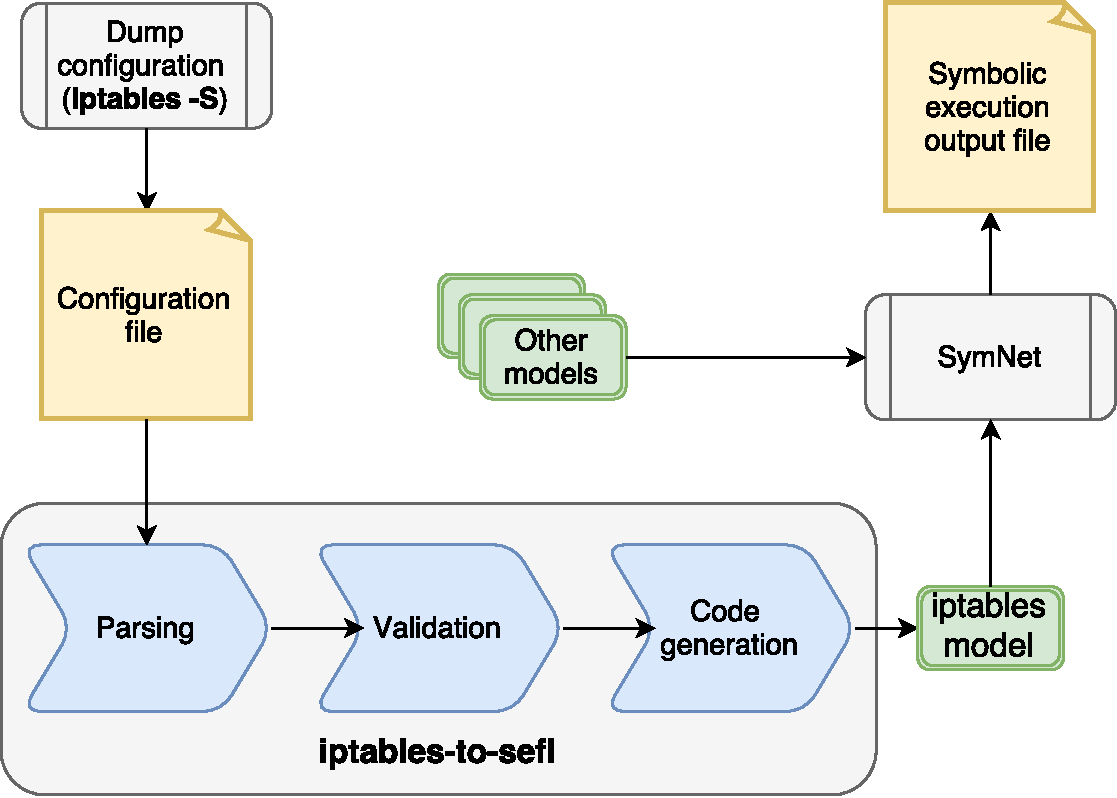
\includegraphics[scale=0.5]{src/img/high-level-design}
  \caption{High-level design of tool iptables-to-sefl.}
  \label{fig:high-level-design}
\end{figure}

Feeding the resulted model to SEFL, possibly alongside models of other network
elements, can be regarded as a fourth step and is included in
\labelindexref{Figure}{fig:high-level-design} which is a high-level overview of
how our tool fits in the big picture of network verification using SymNet.
Similarly, dumping the configs can be considered step zero.

Nodes in AST are called \textbf{IptElement}s.  The class hierarchy that makes
the core of \TOOL is presented in \labelindexref{Figure}{fig:ipt-hierarchy}.
It is a proper use of the composite design pattern in which multiple classes
are both \emph{components} and \emph{composites} at the same time (e.g.
\emph{Chain}, \emph{Rule}, \emph{NegatedMatch}).  ASTs follow the aggregation
relationships.  As with code generation, the only (concrete) types that can
change are the leaves: the matches and the targets that make up the rules.

In addition to the AST types that are used throughout all three computation
phases of our tool, it is worth introducing the class hierarchy behind our
model template too.  It is designed to clearly separate each component (i.e.
\emph{virtual device}) that we identified in the previous chapter and to make
their interconnection as smooth as possible. They are described in more detail
in \labelindexref{Section}{sec:codegen}, but the important thing to notice is
that it \emph{inherits} the composite pattern approach from our core AST
hierarchy.

\clearpage
\begin{figure}[h]
  \centering
  % \captionsetup{justification=centering}

  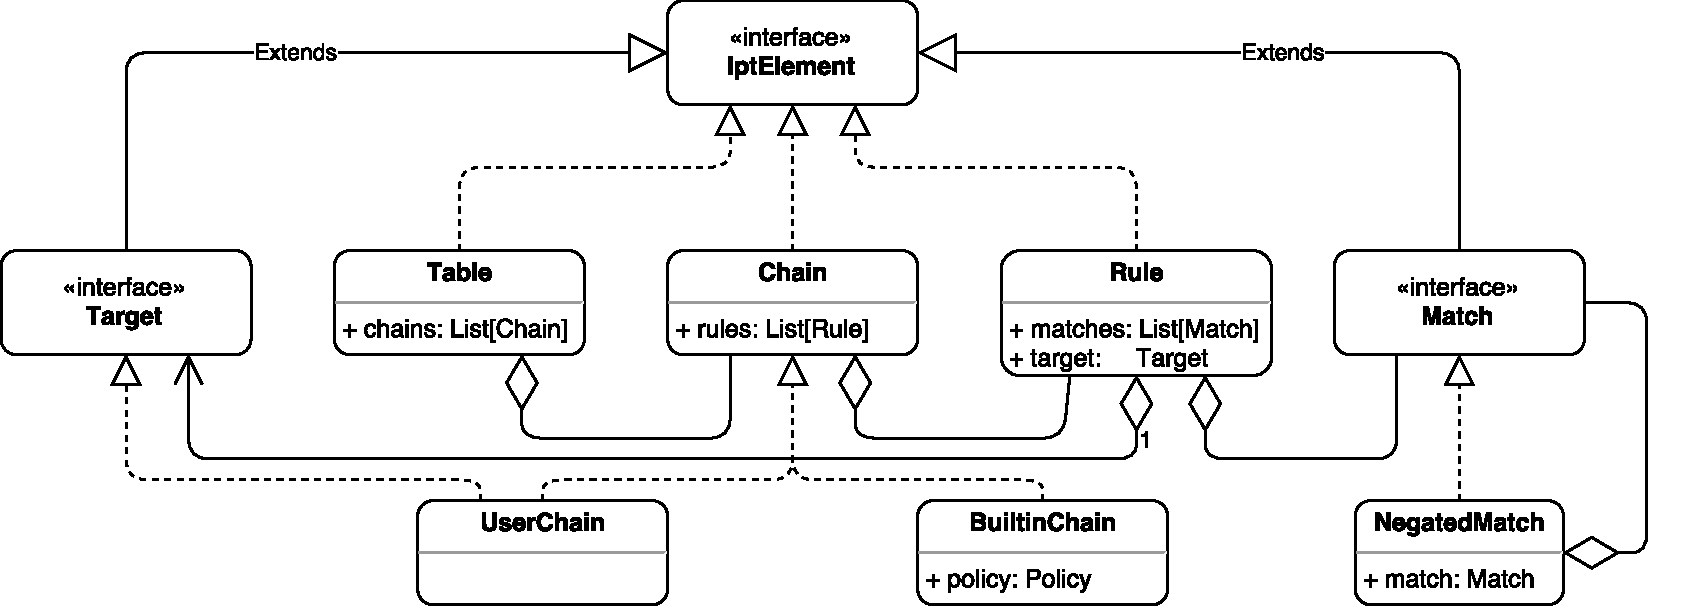
\includegraphics[scale=0.5]{src/img/ipt-hierarchy}
  \caption[The core class hierarchy in iptables-to-sefl.]{The core class
  hierarchy in iptables-to-sefl.  Interfaces \emph{Target} and \emph{Match} are
  the ones that must be subclassed when adding extensions.  The
  \textbf{NegatedMatch} class is a utility class to conveniently negate another
  \emph{Match} instance.}
  \label{fig:ipt-hierarchy}

  \vspace*{\floatsep} % https://tex.stackexchange.com/q/26521/5764

  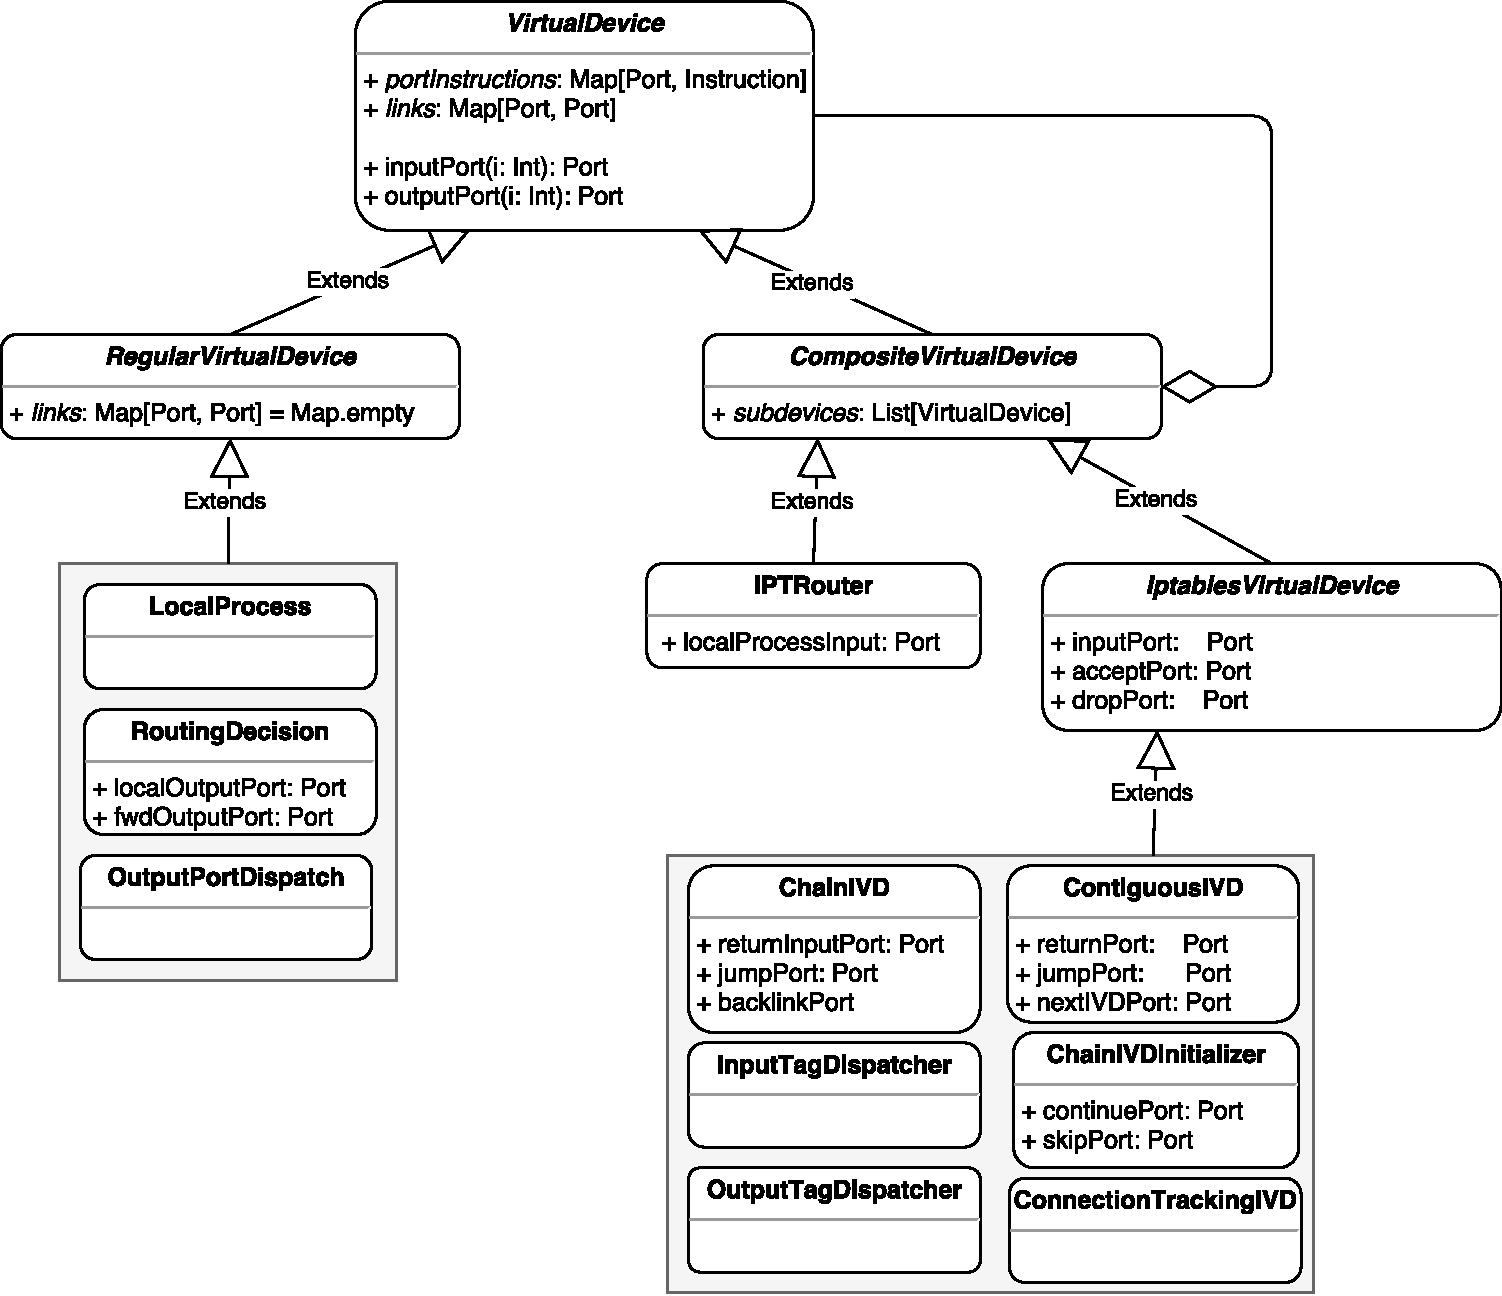
\includegraphics[scale=0.55]{src/img/virtdev-hierarchy}
  \caption[The class hierarchy of the model template part in
  iptables-to-sefl.]{The class hierarchy of the model template part in
  iptables-to-sefl. Besides the abstract base class \emph{VirtualDevice}, there
  are three other classes designed for components with certain expectations:
  \emph{RegularVirtualDevice} for self-contained ones,
  \emph{CompositeVirtualDevices} for components that might built upon some
  other ones, and \emph{IptablesVirtualDevice} for components that implement
  \emph{"iptables"} logic: receive packets, traverse list of rules and apply
  target, which might result in an \emph{accept} or a \emph{drop}.}
  \label{fig:virtdev-hierarchy}
\end{figure}
\clearpage

On top of the compiler-like internal structure, \TOOL features an
\textbf{extension-oriented design} that aims to ease as much as possible the
addition of new extensions. Since iptables supports over 100 official match and
target extensions, it is unrealistic to cover all of them upfront, in a
inextensible, monolithic design.  Even if we could, that is still not
advisable, as it is error prone and hard to debug or refactor.  To add to that,
netfilter itself is built around the idea of seamless extensibility.
Therefore, while it does not happen to often, new, fresh extensions can be
added anytime.

The building blocks of this design are the interfaces \emph{Target} and
\emph{Match} (pedantically, Scala traits), on one hand, and a generic rule
parser that can be \textbf{injected} user-defined parsers for newly added
targets and matches, on the other hand.  They are applied in the order given as
part of the \emph{ParsingContext} object.  This object gets passed and updated
during parsing and is further discussed in the section dedicated to the parsing
phase below.


\section{Parsing}\label{sec:parsing}
* !!!! this makes me thing that I should present the AST components before the
Parsing section.  I was afraid I won't be able to discuss anything in the
parsing section, but there are some things: monadic parser, rule parser (with
match activation), etc.
\todo{grammar of iptable rules, "our" version}
\todo{talk about parsing, table parsing, chain parsing, ParsingContext, rule
parsing, match/target parsing, their extensions, how they are extended, etc}
\todo{for rule parsing, mention the functionality behind the 'match extension
activation', flag -m or --match}
\todo{Monadic, Parsec, functional, haskell etc}


\section{Validation}
\todo{WHY it is needed; say that it is analogous to semantic analysis in
compilers}
\todo{use cases: unordered chains (needed), port range validity, certain chains
in certain tables, certain rules in certain tables/chains, etc}
\todo{how it works, validate() function, validateIf variant, ValidationContext}


\section{Code generation}\label{sec:codegen}
Things to say:
* how components featured in Figures X Y are organized at a high-level but more
implementation-focused (i.e. hierarchy of classes).  Also mention the composite
pattern and that it helps make sure that no internal device is skipped when
adding the links and SEFL instructions to the two Maps that have to result.
\todo{(kind of the same thing as above) add implementation-detailed diagrams of
the 'iptelement' hierarchy as well as of the 'virtualdevice' hierarchy; mention
composite approach, etc.}

\todo{SeflGenOptions trait, the variant for match extensions and the one for
target extensions}


\section{Code structure}

Now that we clarified the implementation challenges we encountered in each of
the three phases that make up our tool and showed how we solved them, let us
briefly present the physical structure and organization of this project.

As most Scala projects, the test suites are separated from the source code: the
former reside in \hlmath{src/test} while the latter fills the \hlmath{src/main}
directory.  Both of these subtrees share the same structure.  Each one of them
sums up to approximately 4k LOC (so a total of \textbf{8k LOC}), while the
dominant paradigm used is \textbf{functional programming}, as already indicated
in the previous sections.

Even if seemingly tightly bound to SymNet, \TOOL has been developed as a
standalone project.  In fact, even though not so obvious from SymNet's internal
structure, we only interact with it through a \textbf{public}
API\abbrev{API}{Application Programming Interface} that exposes the following
components:
\begin{itemize}
  \item The \emph{Instruction} class hierarchy that allows us to generate SEFL
    code.  \labelindexref{Table}{tab:sefl-instr} is a summary of the most
    common instructions we use.
  \item The \emph{Expression} class hierarchy that allows us to express
    \emph{Constraints}.  It includes equality expressions, logical expressions,
    etc.
  \item The \emph{canonical names} module that simplifies the way we refer to
    fields in packet headers, which is especially useful since one of the
    features in SEFL is \emph{guaranteed memory safety}.
  \item The \emph{execution context} module that provides a very simple and
    intuitive interface to run symbolic execution on a given model.
\end{itemize}

\begin{listing}
  \lstset{numbers=none, frame=single, basicstyle=\ttfamily,
    xleftmargin=0.30\textwidth, xrightmargin=0.30\textwidth
  }
  \begin{lstlisting}
core/
extensions/
virtdev/
Driver.scala
package.scala
  \end{lstlisting}
  \caption{Contents of the relevant source code subdirectory.}
  \label{lst:root-directory}
\end{listing}

The root of the actual source directory is shown in
\labelindexref{Listing}{lst:root-directory}.  The \hlmath{core/} directory
contains the \textbf{IptElement} class hierarchy
(\labelindexref{Figure}{fig:ipt-hierarchy}), the monadic base parsers discussed
in \labelindexref{Section}{sec:parsing}, and the generic parsers for tables,
chains and rules.  The \hlmath{extensions/} directory has one subdirectory for
each extension supported.  Each one of them defines custom \emph{Target}s
and/or \emph{Match}es alongside their corresponding parsers.  The
\hlmath{virtdev/} directory contains the model template class hierarchy
(\labelindexref{Figure}{fig:virtdev-hierarchy}) and all the logic discussed in
\labelindexref{Section}{sec:codegen} for putting all chains and tables
together.  \textbf{Driver} is a class that sequentially runs the three phases
and outputs all explored execution paths.  It makes use of the \emph{execution
context} exposed by SymNet.  Finally, \textbf{package.scala} is a file that
defines various package-level utility functions and/or constants.


\section{Extension examples}
\subsection{TCP and UDP}
\subsection{MARK and CONNMARK}
